\section{Mason}

MASON (Multi-Agent Simulation of Neighbourhoods, or Networks) is a versatile Java library for providing the key architecture in agent-based applications. MASON provides a range of environment representations, or \textit{fields} in MASON nomenclature, and a GUI system that intuitively visualises system components that interact in and with the MASON fields.

This project did not tie itself heavily to MASON's broad range of features. MASON only provided a very lightweight framework to act as a foundation for the simulation construction: MASON fundamentally revolves around a \code{Schedule} object, which is an enhanced priority queue. For an agent to act in the system it must inherit the \code{Steppable} interface, which guarantees the agent has a \code{step()} method. Agents are queued into the \code{Schedule} for each time step, and the \code{Schedule} executes the agent's step method when it reaches the top of the queue. In compliment with this simple functionality, the \code{Schedule} will step higher priority agents first and will step agents of equal priority in a uniformly random order.

In addition to the \code{Schedule}, MASON's other contribution to the project was providing a GUI, and MASON's GUI-compliant graph data structure functionality. A MASON \code{Network} is a simple collection of arbitrary user-defined objects to use as nodes, and a map between nodes and their associated edge objects. While MASON expects users to provide a class to act as a node, it provides its own \code{Edge} class. \code{Edge} objects store a `from node', `to node' and an arbitrary user-defined child object, which is expected to store semantic data about what the edge represents in the context of the simulation. MASON networks hence act as wrappers for user-defined node and edge objects - to that end, \code{Junction} objects were defined as the \code{Network}'s node objects, and \code{Road} objects were constructed to provide a semantic representation of roads in the simulation. The driving reason for using a MASON \code{Network} rather than constructing a graph directly from the \code{Junction} and \code{Road} objects is the ease of the MASON network integration with MASON's own GUI and visualisation tools. Using MASON's effective UI framework allows more focus to be directed towards the core system design, and the evaluation of evacuation strategies.


\section{System Overview}

At the highest level, the project is composed of a simulation package, working in tandem with MASON, and a collection of classes which leverage the simulation package. Figure \ref{fig:system_overview} gives a simple class-relationship diagram of the system which articulates this high-level package split as well as portraying a lower level system composition; the simulation package consists of a set of agents, a collection of environment classes, a pair of classes for implementing the A* algorithm, and most importantly, the \code{CoreSimulation} class. A brief overview of each component is listed in Table \ref{tab:simcomponents}.

\begin{figure}[]
    \centering
    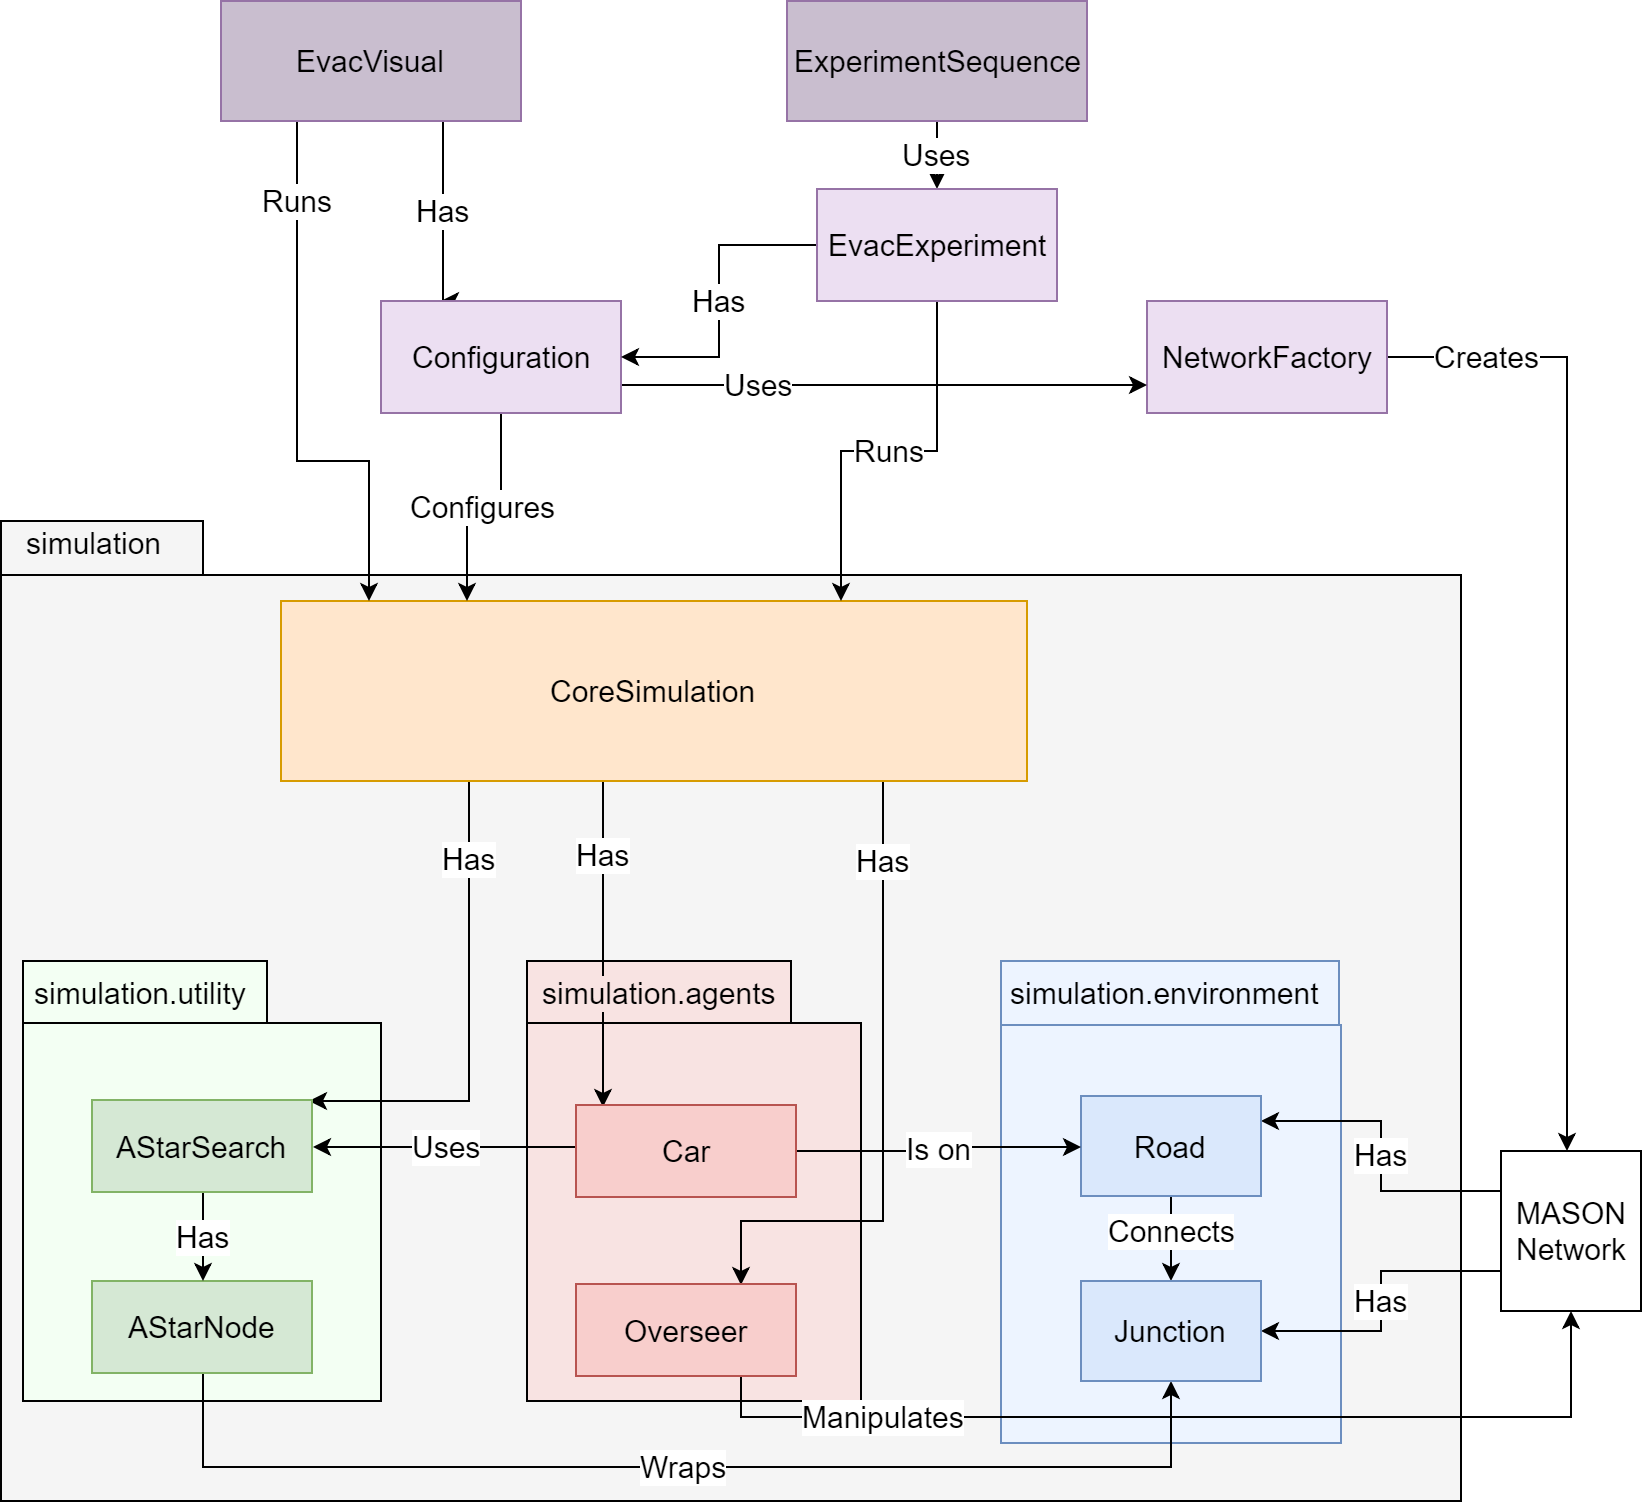
\includegraphics[width=0.95\linewidth]{images/system_overview.png}
    \caption{Project component relationship diagram}
    \label{fig:system_overview}
\end{figure}

\code{CoreSimulation} is the backbone of the program - it sets up the virtual environment, constructs a population of agents and populates the system with them. \code{CoreSimulation} extends MASON's \code{SimState} class, which is the central class in the framework. \code{SimState} provides the Schedule and a Java implementation of the \textit{Mersenne Twister} random number generator by Matsumoto and Nishimura (1998), which performs far better than java.util.Random \cite{Matsumoto1998MersenneGenerator,TylerSunRandomness}. Note that Figure \ref{fig:system_overview} does not include any references to MASON objects, with the exception of the \code{Network} class which is integral to the relationships between the simulation, the agents, and the road network proper - a full UML class diagram with MASON superclasses and interfaces is available at Appendix \ref{appendix:class_diagram}.

\begin{sloppypar}
The \code{SimplePortrayal2D} class is a MASON GUI class. By extending this class, MASON will intuitively be able to visualise an object in the UI. \code{SimplePortrayal2D.draw(...)} can be overridden to customise the object's visual appearance.
\end{sloppypar}

\begin{table}[]
\centering
\makebox[\textwidth][c]{%
\begin{tabularx}{1.1\textwidth}{@{}lXl@{}}
\toprule
Class                 & Description                                                                                                                                                                                                     & Class Inheritance                                                                                         \\ \midrule \addlinespace[0.2cm]
\code{CoreSimulation} & \begin{tabular}[c]{@{}l@{}}The simulation proper\\ Stores environment fields and agents\end{tabular}                                                                                                            & Extends \code{SimState}                                                                                   \\ \addlinespace[0.2cm]
\code{Car}            & Implementation of car agents. Their step function evaluates their environment and attempts to move towards their evacuation goal                                                                                & \begin{tabular}[c]{@{}l@{}}Implements \code{Steppable}\\ Extends \code{SimplePortrayal2D}\end{tabular} \\ \addlinespace[0.2cm]
\code{Overseer}       & Implementation of overseer agents. An Overseer checks the network at every step and throttles roads according to the throttling rules given in Chapter \ref{ch:background}.                                     & \begin{tabular}[c]{@{}l@{}}Implements \code{Steppable}\end{tabular}         \\ \addlinespace[0.2cm]
\code{Junction}       & Networks are defined by Junctions connected by MASON \code{Edge} objects.                                                                                                                                       & Extends \code{SimplePortrayal2D}                                                                          \\ \addlinespace[0.2cm]
\code{Road}           & Mason \code{Edge} objects wrap a \code{Road} object. \code{Road}s have lengths, a record of all traffic on them and a reference to their source and destination \code{Junction}s.                               &                                                                                                           \\ \addlinespace[0.2cm]
\code{AStarSearch}    & A utility class which Cars use to find shortest evacuation paths                                                                                                                                                &                                                                                                           \\ \addlinespace[0.2cm]
\code{AStarNode}      & This wrapper class is used to track heuristic data for each \code{Junction}, which is required by the A* algorithm, without cluttering the \code{Junction} class which has no direct need for owning such data. &                                                                                                           \\ \bottomrule
\end{tabularx}%
}
\caption{Simulation class component descriptions}
\label{tab:simcomponents}
\end{table}

\section{Running Simulations}

\code{ExperimentSequence} and \code{EvacVisual} are two ways for a user to interact with the simulation. \code{ExperimentSequence} is designed to be used in the context of research, it executes a batch of experiments. EvacVisual runs a single simulation with visualisation.

\code{ExperimentSequence} is run with an input list of simulation configuration XML files, each corresponding to an individual experiment. Each experiment is handled by a an \code{EvacExperiment} object which manages iteration across the examined space of independent variables, and takes repeat measurements. Configuration file parsing functionality is performed by a \code{Configuration} object. 

\code{EvacVisual} also uses a \code{Configuration} object, as it requires a simulation configuration file to run, but it does not sequence multiple simulations or record any data. The program opens two windows on launch, the console (Figure \ref{fig:gui_console}) and the display window (Figure \ref{fig:gui_display}.

\begin{figure}
    \centering
    \begin{subfigure}[b]{0.5\textwidth}
        \centering
         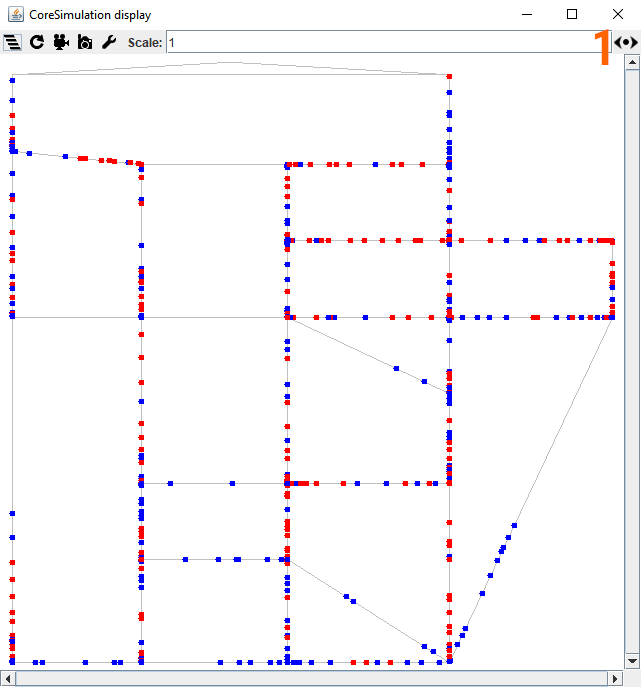
\includegraphics[width=\textwidth]{images/display_edit.png}
         \caption{Simulation display window}
         \label{fig:gui_display}
    \end{subfigure}
    \hspace{1cm}
    \begin{subfigure}[b]{0.3\textwidth}
        \centering
         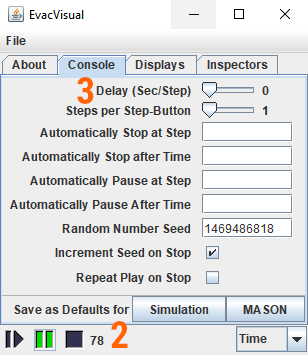
\includegraphics[width=\textwidth]{images/console_edit.png}
         \caption{Simulation console window}
         \label{fig:gui_console}
    \end{subfigure}
    \caption{Annotated images of the \textit{EvacVisual} simulation visualisation components}
    \label{fig:gui}
\end{figure}

\subsubsection{Display}
This window shows the simulation in progress.

Roads are drawn as thin grey lines, if a road is throttled it is drawn in red. Cars are drawn as circles; typically red but coloured blue if they are \textit{greedy} agents. Image zoom can be adjusted by the buttons in the top-right (Figure \ref{fig:gui}: \textit{label 1}) and  when zoomed in the scroll bars can direct the camera view.

\subsubsection{Console}

MASON's console feature provides a collection of interfaces that interact with the visualisation. Many of these interfaces have limited use, but some are crucial - most importantly is the lower tray of buttons (Figure \ref{fig:gui}: \textit{label 2}). The contents of the tray are, from left to right: manual step button; pause/play button; stop-and-reset button; time/step counter. The time/step counter can be changed using the bottom-right dropdown menu. An additional console feature of high importance is the \textit{Delay} scale (Figure \ref{fig:gui}: \textit{label 3}). Naturally the EvacVisual program will run as fast as the processor allows it, adding a time delay between each advancing step slows down the animation to become comprehensible. By default, the time resolution of the system is 1 step/second, so a Delay of 1 would run the simulation at `real-time'. 